%% Chapter 5 %%%
\chapter[Ошибка базовой оценки]{\emph{Р}-значение и ошибка базовой оценки}
\label{chp5}
\chaptermark{Ошибка базовой оценки}

Как вы уже видели, \emph{р}-значения интерпретировать непросто. То, что мы получили статистически незначимые результаты, не означает, что различий не существует. А что означает статистически значимый результат?

Давайте посмотрим на примере. Предположим, я решил протестировать сотню потенциальных лекарств от рака. Только десять из них реально действуют, но я не знаю, какие именно - мне нужно проводить эксперименты, чтобы определить это. В самих экспериментах, я буду ориентироваться на $p<0,05$ в оценке различий с действием плацебо, что будет демонстрировать полезность тестируемого лекарства. 

Для иллюстрации, на изображении ниже каждая клетка таблицы представляет собой одно лекарство. Синим отмечены те клетки, которые соответствуют действующим лекарствам:


%\newpage % делаем разрыв, чтобы картинка была первой на след странице

%%%%%%%%%%%%%% figure 5 %%%%%%%%%%%%%%%%%%5
\begin{figure}[h!]
    \centering
    
\includegraphics[width=0.4\textwidth]{drug-grids-1}
    %\caption{}
    \label{fig5:drug-grid-1}
\end{figure}
%%%%%%%%%%%%%%% end of figure 5 %%%%%%%%%%%%%%%%%%%

Как мы видили ранее, в большинстве испытаний сложно определить каждое хорошее лекарство. Давайте предположим, что статистическая мощность моих тестов - 0,8. Из десяти действующих лекарств, я смогу правильно распознать примерно 8 (отмечены фиолетовым на иллюстрации ниже):

\newpage % делаем разрыв, чтобы картинка была первой на след странице

%%%%%%%%%%%%%% figure 6 %%%%%%%%%%%%%%%%%%5
\begin{figure}[h!]
    \centering
    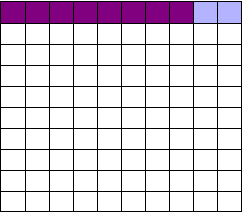
\includegraphics[width=0.4\textwidth]{drug-grids-2}
    %\caption{}
    \label{fig5:drug-grid-2}
\end{figure}
%%%%%%%%%%%%%%% end of figure %%%%%%%%%%%%%%%%%%%


Я также предположу, что около 5 из 90 недействующих лекарств будут иметь значимые эффекты. Почему? Напомню, что \emph{p}-значение подсчитывается исходя из предположения об отсутствии эффекта, т.е. $ p =0,05$ означает, что существует 5\% шанс сделать ошибочный вывод о том, что недействующее лекарство на самом деле действует.

Таким образом, я провожу свои эксперименты и делаю вывод о том, что у меня есть 13 действующих лекарств: 8 хороших лекарств и 5 тех, что я мог ошибочно включить в свой список (показаны красным на илюстрации ниже):


%\newpage % делаем разрыв, чтобы картинка была первой на след странице

%%%%%%%%%%%%%% figure 6 %%%%%%%%%%%%%%%%%%5
\begin{figure}[h!]
    \centering
    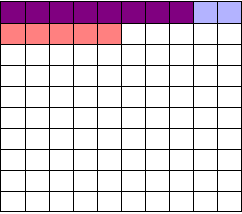
\includegraphics[width=0.4\textwidth]{drug-grids-3}
    %\caption{}
    \label{fig5:drug-grid-3}
\end{figure}
%%%%%%%%%%%%%%% end of figure %%%%%%%%%%%%%%%%%%%

Шанс того, что любое из ``действующих'' лекарств будет действительно эффективным, составляет только 6\%. Если бы я случайным образом выбрал одно лекарство из ста, провёл на нем свои тесты и обнаружил бы статистически значимую связь на уровне $p<0,05$, то существует всего 62\% шанса на то, что это лекарство действительно эффективно. Говоря терминами статистики, мои шансы совершить ошибку первого рода (оценка ложной тревоги) - это доля ложных положительных результатов в общем количестве статистически значимых результатов - составляют 38\%.  

Поскольку базовая оценка эффективности лекарств от рака довольно низкая - только около 10\% от множественных испытаний и лекарств дают какой-то результат, - большинство из тестируемых лекарств не действуют, и мы становимся особенно уязвимы к совершению ошибки первого рода. Будь я полным неудачником и будь у меня хоть целый грузовик совершенно бесполезных лекарств, базовая оценка эффективности которых составляет 0\%, я бы имел 0\% шанса на получение хоть какого-либо статистически значимого результата. Тем не менее, я все равно получу результат в $p<0,05$ для 5\% этих лекарств.

Часто можно слышать, как люди приводят в пример \emph{p}-значения в качестве показателя малой вероятности получения ошибки. ``Существует только 1 шанс из 10000, что такой результат возник случайным образом'' - говорят они, потому что получили значение $p=0,0001$. Увы, нет! Такое утверждение игнорирует базовую оценку, и встречается под названием \emph{ошибка базовой оценки}. Напомним, как определяется \emph{p}-значение:

\begin{quotation}

\textbf{\emph{P}-значение} можно определить как вероятность получить результат равный или больший, чем в реальности наблюдаемый, при условии, что никакого эффекта или различий обнаружено не было (нулевая гипотеза).   

\end{quotation}


\emph{P}-значение рассчитывается, основываясь на предположении о том, что лекарство \emph{не действует}, и даёт нам вероятность получения данных равных или больше тех, что мы получили. Оно не даёт нам вероятность того, что лекарство действует.

Когда кто-либо использует полученные \emph{p}-значения в качестве доказательства того, что они правы, запомните это. Вероятность ошибки их исследования, скорее всего, довольно высока. В сферах, где большинство проверяемых гипотез опровергаются, как, например, в первичных тестах лекарств (большинство таких лекарств не проходят тесты), вполне вероятно, что большинство ``статистически значимых'' результатов с $p < 0,05$ на самом деле всего лишь случайность.

Отличный пример тому - тесты на медицинскую диагностику.


\section[В медицинских испытаниях]{Ошибка базовой оценки в медицинских испытаниях}
\label{chp5:base-rateF}
\sectionmark{Медицинские испытания}

Существуют некоторые разногласия во мнениях по поводу использования маммографии при тестировании на рак груди. Некоторые считают, что опасность получить ложноположительный результат (и последующие ненужные биопсия, хирургическое вмешательство и химиотерапия) превышает те преимущества, которые даёт раннее обнаружение рака. Это статистический вопрос, давайте попробуем дать оценку.

Предположим, что у 0,8\% женщин, которым предписали маммографию, действительно  рак груди. У 90\% женщин, имеющих рак груди, маммография сможет его обнаружить. (Это статистическая мощность теста, но приблизительная, поскольку очень сложно сказать, сколько случаев рака груди мы упустили, если мы не знаем, что они вообще есть.) Тем не менее, из женщин, не имеющих рака груди, около 7\% получат ложноположительный результат на маммографии, ведущий к дальнейшим тестам, лечению и биопсии. Если вы получили положительный результат маммографии, каковы шансы на то, что у вас действительно рак груди?

Опуская те ситуации, когда ты, читатель, мужчина\footnote{Забавно, но если вы - мужчина, это не исключает возможности получить рак груди; это лишь делает вероятность чрезвычайно малой.}, ответ - 9\%.\cite{kramer_how_2005}

Несмотря на то, что тест даёт ложноположительный результат лишь у 7\% женщин, не имеющих рак груди, что аналогично $p < 0,07$, порядка 91\% положительных результатов на самом деле ложноположительные.

Как я это рассчитал? Точно таким же методом, как и в примере про лекарство от рака. Представьте себе 1000 случайно выбранных женщин, которые решили пройти маммографию. У восьми из них (0,8\%) есть рак груди. Маммография обнаруживает правильно около 90\% случаев рака, т.е. примерно у семи из восьми женщинрак будет обнаружен. Однако, остается 992 женщины без рака груди, и 7\% из них получат ложноположительный результат, т.е. у 70 женщин будет неверно диагностирован рак груди.

В сумме у нас получается 77 женщин с положительным результатом маммографии, у 7 из которых действительно есть рак груди. Только у 9\% женщин с положительным результатом по маммографии действительно есть рак груди.

Если задать этот вопрос студентам, изучающим статистику, и преподавателям научной методологи, более трети из них не смогут ответить верно.\cite{kramer_how_2005} Если задать его врачам, две трети из них провалятся на этом вопросе.\cite{bramwell_health_2006} Они ошибочно делают вывод о том, что $p < 0,05$ означает 95\% вероятность того, что результат истинный, хотя, как вы можете видеть из приведённых примеров, вероятность того, что положительный результат истиннен, зависит от того, какая часть проверенных гипотез верна. И нам просто повезло, что в любой момент времени рак груди возникает лишь у небольшой части женщин. 

Пролистайте вводные учебники по статистике и вы встретите подобное заблуждение довольно часто. \emph{P}-значения трудны для понимания, а ошибка базовой оценки встречается повсеместно.  


\section{Оружие против ошибки базовой оценки}
\label{chp5:arms-baserateF}
\sectionmark{Оружие против ошибки базовой оценки}

Чтобы столкнуться с этой ошибкой, нет нужды проводить расширенное исследование или тестировани на рак. А что, если вы делаете социологическое исследование? Например, вы хотите опросить американцев, чтобы узнать как часто они используют оружие в целях самообороны. В конце концов, в основе аргументов сторонников контроля оружия находится именно право на самозащиту, поэтому важно определить, используется ли оружие в большинстве случаев для защиты и перевешивает ли это недостатки, например, убийства.

Один из способов собрать необходимые данные - опрос. Можно опросить репрезентативную выборку американцев, узнав, владеют ли они оружием, и если да, использовали ли когда-нибудь оружие для защиты своего дома от незаконного проникновения или для защиты себя от ограбления. Затем можно сравнить полученные данные со статистикой правоохранительных органов об использовании оружия в случаях убийства и сделать вывод на основании этого вывод.

Такие опросы уже проводились, и результаты их довольно интересные. Один телефонный опрос, проведенный в 1992 году, позволил оценить, что американские граждане используют оружие в целях самообороны до 2,5 миллиона раз ежегодно - то есть, около 1\% американских взрослых защищали себя с помощью оружия. В 34\% случаях это была защита от незаконного проникновения в жилище, т.е. порядка 845000 взломов было остановлено владельцами оружия. Но за 1992 год было совершено только 1,3 миллиона взломов в дома, в которых кто-либо был. Две трети из них произошли в тот момент, когда жильцы дома спали, и сам факт взлома и ограбления был обнаружен уже после того, как воры покинули жилище. Получается, что остается порядка 430000 случаев взлома, когда домовладельцы были в доме и противостояли грабителям и, как нас пытаются убедить, в 845000 случаях из них, грабители были остановлены жителями - владельцами оружия.\cite{hemenway_survey_1996}   


Ой!


Что произошло? Почему опрос переоценил количество случаев использования оружия в целях самозащиты? По тем же причинам, что и маммография давала завышенную оценку случаев рака груди: гораздо больше возможностей для ложноположительных результатов, чем ложноотрицательных. Если 99,9\% людей никогда не использовали оружие в целях самообороны, но 1\% из них ответит ``да'' на любой вопрос просто ради забавы, еще 1\% ответит так, чтобы выглядеть более мужественно, а 1\% просто неправильно поймёт вопрос, - вы получите значительную переоценку использования оружия в целях самозащиты.

А что насчет ложноотрицательных результатов? Могут ли они быть сбалансированы людьми, которые говорили ``нет'', даже если они лично застрелили грабителя на прошлой неделе? Ответ: нет. Если лишь немногие действительно используют оружие в качестве самообороны, тогда возможность получить ложноотрицательные результаты слишком низка. Они вытесняются ложноположительными результатами.

Эта ситуация аналогична примеру с лекарствами от рака, описанному ранее. Здесь \emph{p}-значение - это вероятность того, что кто-нибудь будет ошибочно утверждать, что он использовал оружие в целях самообороны. Даже если значение \emph{p} будет небольшим, ваш окончательный ответ будет все равно неверным. 


Чтобы снизить \emph{p}-значение, криминологи используют более детальные опросы. Например, в исследованиях показателя национальной виктимизации населения (NCVS) используются подробные сидячие интервью с исследователями, где респондентов спрашивают о деталях преступлений и использования ими оружия в целях самообороны. Чем больше подробностей в опросе, тем лучше исследователи могут оценить, подходит ли конкретный инцидент под критерии самообороны. Результаты таких исследований гораздо скромнее - около 65000 случаев в год. Существует вероятность того, что эта оценка занижена, но и меньший шанс массовой переоценки.     


\section[Не удалось в первый раз - пробуйте еще]{Не удалось в первый раз - пробуйте еще}
\label{chp5:try-again}

Ошибка базовой оценки показывает, что ложноположительные результаты более вероятны в том случае, если вы считаете $p < 0,05$ критерием значимости. Большинство современных исследований не полагается только на один показатель значимости - они сравнивают эффекты нескольких факторов, надеясь найти один с наиболее значимыми эффектами.

Например, представьте себе исследование, в котором проверялось бы, являются ли драже причиной появления угревой сыпи на коже, путём исследования эффекта драже различного цвета: %см. \hyperref[fig5:xkcd-significant]{комикс xkcd}.

\newpage % делаем разрыв, чтобы картинка была первой на след странице

%%%%%%%%%%%%%% figure 7 %%%%%%%%%%%%%%%%%%5
\begin{figure}[h!]
    \centering
    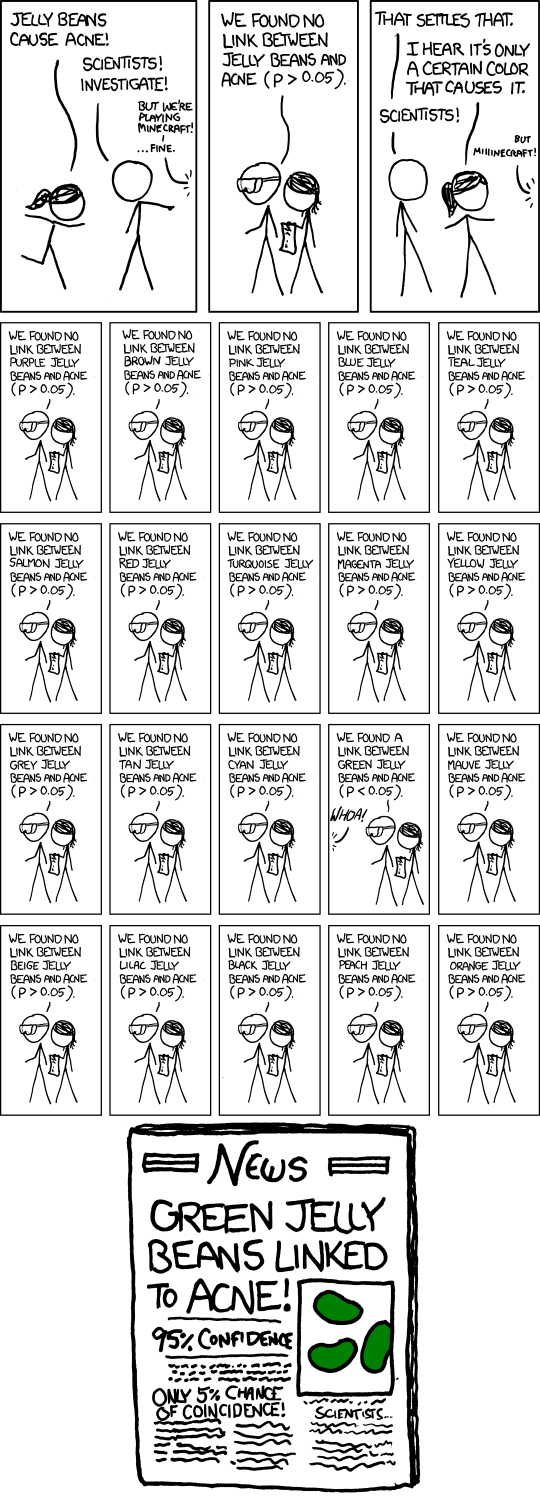
\includegraphics[width=0.5\textwidth]{xkcd-significant}
    \caption{xkcd-комикс, автор Randall Munroe. \href{http://xkcd.com/882/}{http://xkcd.com/882/}}
    \label{fig5:xkcd-significant}
\end{figure}
%%%%%%%%%%%%%%% end of figure %%%%%%%%%%%%%%%%%%%

Как видите, множественные сравнения подразумевают большое количество шансов получить ложноположительный результат. Например, если я буду исследовать 20 разных по вкусу драже, которые никаким образом не являются причиной появления угревой сыпи, и буду искать корреляцию с уровнем значимости $p < 0,05$, у меня будет 64\% шанс получить ложноположительный результат.\cite{smith_impact_1987} Если я проверю 45 различных драже, этот шанс вырастет до 90\%.

Множественные сравнения делать легко, и необязательно для этого, например, тестировать 20 потенциальных лекарств. Попробуйте отследить симптомы дюжины пациентов в течении дюжины недель и проверьте значимые различия в любой момент времени и вы получите 12 сравнений. Попробуйте проверить появление 23 потенциально опасных побочных эффекта и всё - вы уже согрешили. Разошлите десятистраничный опросник, выясняющий отношение людей к строительству атомной электростанции, потребление молока, возраст, количество кузенов, любимую пиццу, цвет носков и множество других хорошо измеряемых факторов, и вы найдете что-нибудь, что вызывает рак. Просто задайте достаточное количество вопросов, и обязательно что-нибудь найдётся.

Опрос на тему медицинских испытаний, проведённый в 1980-х, выявил, что за одно испытание, в среднем, делается около 30 терапевтических сравнений. В более чем половине испытаний исследователи делали настолько много сравнений, что вероятность получить ложноположительный результат была очень высока, а статистическая значимость результатов, о которых они сообщали, подвергалась сомнению: они, возможно, получали статистически значимые эффекты, но это могли быть и ложноположительные результаты.\cite{smith_impact_1987}

Существуют техники, позволяющие корректировать результаты в случае множественных сравнений. Например, метод коррекции Бонферрони утверждает, что если вы делаете $n$ сравнений в испытании, ваш критерий значимости должен быть $p < 0,05/n$. Это понижает шанс получить ложноположительный результат, по сравнению с ситуацией, когда вы делаете только одно сравнение на уровне $p < 0,05$. Однако, как можно себе представить, это снижает статистическую мощность, поскольку вам понадобятся более высокие кореляции для вывода о том, что они статистически значимы. Это сложный компромисс, и катастрофически малое количество статей его когда-либо вообще принимали во внимание.


\section{Ложный след в сканировании мозга} % английская идиома http://en.wikipedia.org/wiki/Red_herring 
\label{chp5:redherrings}

Нейроученые обычно делают огромное количество сравнений. Они часто проводят исследования с использованием фМРТ\footnote{Функциональная магнитно-резонансная томография}, где сравниваются трёхмерные изображения мозга, сделанные до и после того, как испытуемые выполняли какое-либо задание. Эти изображения показывают кровоток в мозгу, что позволяет выявить, какие участки мозга были наиболее активны в момент выполнения задания.

Но как определить, какие именно участки мозга были активны во время выполнения задания? Есть простой способ - разделить изображение мозга на небольшие кубические элементы, называемые вокселами. Воксел из изображения ``до'' сравнивается с вокселом из изображения ``после'', и если различия в кровотоке значительны, можно сделать вывод о том, что эта часть мозга была активна в момент выполнения задания. Проблема, однако, заключается в том, что сравниваемых вокселов - тысячи, а значит существует большой шанс получить ложноположительный результат.

В одном исследовании, к примеру, изучались эффекты ``умственного задания, допускающего неограниченное количество решений''. Участникам эксперимента показывали ``серию фотографий, на которых были изображены человеческие особи в социальных ситуациях с определенной эмоциональной валентностью,'' и просили их ``определить, какую эмоцию испытывает изображенный на фотографии субъект.'' Можете себе представить, насколько разные эмоциональные и логические центры мозга могли быть активными в процессе решения этого задания.   

Данные были проанализированы, и были замечены определенные участки мозга, изменяющие свою активность в процессе выполнения задачи. Сравнение изображений ``до'' и ``после'' дало различие на уровне значимости $p = 0, 001$ в 81 мм\textsuperscript{3} кластере мозга.

А участники исследования? Нет, это не были, как обычно, студенты вузов, участвующие в исследовании за 10\$. В качестве испытуемого выступал один 1,8 килограммовый атлантический лосось, который ``на момент сканирования не был жив''. \cite{bennett_neural_2009}  

Естественно, большинство нейронаучных исследований гораздо сложнее этого: существуют методы поиска кластеров вокселов, которые изменяются все вместе и одновременно, а также техники контроля возможных ложноположительных результатов даже в случае, когда проводятся тысячи статистических тестов. На данный момент, эти методы широко распространены в нейронаучной литературе, и те простые ошибки, что я описал, уже не так часто встречаются. Но, к сожалению, практически каждая статья решает проблему по-разному: обзор 241 исследования с использованием фМРТ показал, что в них были использованы 223 уникальные стратегии анализа, что, как мы обсудим позднее, \hyperref[chp8]{даёт огромную гибкость исследователям} получать статистически значимые результаты.\cite{carp_secret_2012}  


\section{Контроль оценки ложноположительных результатов}
\label{chp5:controlfalserate}

Ранее я упоминал, что существуют техники коррекции для множественных сравнений. Метод Бонферрони, например, предполагает, что можно правильно оценить ложноположительные результаты используя $p < 0,05/ n$, где $n$ - это количество статистических тестов, которые необходимо провести. Если проводить исследование, в котором делается двадцать сравнений, вы можете использовать пороговое значение в $p < 0,0025$ для уверенности в том, что есть только 5\% шанс ошибочно признать несуществующий эффект статистически значимым.

Однако, у этого метода есть недостаток. Понижая \emph{p}-значение , необходимое для признания результата статистически значимым, вы значительно понижаете статистическую мощность исследования, и легко можете упустить как реальный эффект, так и ложный. Существуют более сложные, чем коррекция Бонферрони, процедуры, которые используют преимущества определенных статистических свойств проблемы для увеличения статистической мощности, хотя и они не могут совершить магию. 

Хуже то, что они не избавляют вас от ошибки базовой оценки. Полученое \emph{p}-значение все еще может вводить вас в заблуждение, и вы ошибочно будете утверждать, что ``существует лишь 5\% шанс, что я ошибаюсь'', хотя вы лишь ликвидировали некоторые ложноположительные результаты. Ученые в большей степени заинтересованы в оценке ложноположительных результатов: какая часть моих статистически значимых результатов является ложноположительными? Существует ли какой-нибудь статистический тест, позволяющий мне контролировать эту часть? 

В течение длительного времени, ответ на этот вопрос был прост - ``нет''. Как вы видели в разделе об ошибке базовой оценки мы можем примерно оценить количество ложноположительных результатов, если мы предположим, какое количесто проверенных нами гипотез истинны, - однако, мы скорее узнаем это из полученных данных, чем будем угадывать. 

В 1995 году Бенджамини и Хохберг предложили более полезный ответ. Они разработали исключительно простую процедуру, которая может подсказать, какое \emph{p}-значение можно считать статистически значимым. До этого момента я старался избегать математических подробностей, однако цитата ниже иллюстрирует насколько проста эта процедура:

\begin{quotation}
Проведите необходимые статистические тесты и получите для каждого из них \emph{p}-значение. Составьте из них список в порядке возрастания.

Выберите оценку ложно положительных результатов и обозначьте её $q$, а количество статистических тестов $m$.

Найдите такое наибольшее \emph{p}-значение, соответствующее $p <= i*q/m$, где $i$ это порядковый номер \emph{p}-значения в упорядоченном выше списке.

Все \emph{p}-значения меньше или равные этому можно считать статистически значимыми. 
\end{quotation}  

Вот и всё! Процедура гарантирует, что из всех статистически значимых результатов, ложноположительных будет не более $q$ процентов. \cite{benjamini_controlling_1995}


Метод Бенджамини-Хохберга быстр и эффективен, и в определенных сферах стал широко применяться учеными и статистиками. Его использование даёт лучшую статистическую мощность, чем коррекция Бонферрони, кроме того, предоставляя более наглядные результаты. Он может использоваться в различных ситуациях, и варианты этой процедуры дают лучшую статистическую мощность на различных типах данных.

Конечно, метод не идеален. В некоторых странных ситуациях, он даёт довольно глупые результаты, и, как было математически доказано, всегда есть шанс того, что он может оказаться малополезным для контроля оценки ложноположительных результатов. Но это лучше, чем ничего, особенно для начала.
